\chapter{Design and Implementation of Slope}
\label{chap:design}

We then discuss migration and show how it satisfies the above
Then discuss core migration algorithm

\section{Programming model}
\label{sec:platform}

Applications have to call into Slope to \CHECK{} initiate and carry on the
migration operations. Since Slope requires intimate access to the application
memory, we need to choose a low level platform with first class support for
memory management.

We have chosen C++ as the platform to implement Slope, mainly because we need
to directly access process memory and manage the way it is allocated and used.
Whether or not these limitations can be eliminated, for example by using Slope
as a service or like a sidecar process, as opposed to a library are future
research directions.



\subsection{Local memory layout}
Before we can discuss the main components of Slope, we need to discuss how
memory is managed in each application instance which uses Slope. Similar to
RAMP \cite{memon2018ramp}, each program instance \CHECK{Sorry what's the problem with this: reserves} a
large \CHECK{How do you choose the size? Equal to physical memory would be too large.} \TODO{elaborate how large is practical and why. Required for a future section} (e.g. equal to the machine's physical memory size) continuous part
of its virtual memory address space, starting at the same virtual address
on every machine, to be used by Slope.
This is done \CHECK{at} program construction
time (i.e. before \texttt{main()}) \CHECK{and we will refer to} call this section of the virtual
address space the migratable memory or Slope memory. Note that mappings for
these pages are not yet generated and therefore the size of the Slope memory
region can be expanded to the whole 64 bits of address on current machines.
We will manage the slope memory by 4KB page granularity \CHECK{ as this is the
smallest unit of control for setting the protection of memory mappings}.
We do not use \TODO{discuss why you do not need contiguous physical memory}
hugepages or contiguous physical memory as the former results in
loss of granularity and the latter needs to be done from inside the kernel and
typically at boot time before memory fragmentation gets in the way.

\begin{figure}
\centering
\ensurepdffromsvg{local-memory-management-phys-log.drawio}
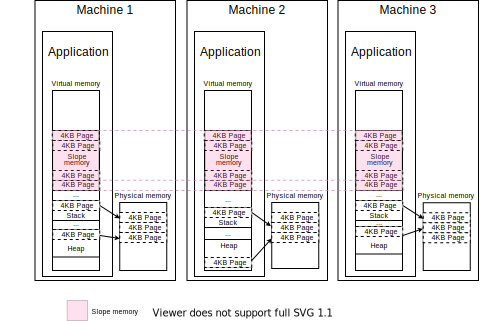
\includegraphics[width=1\textwidth]{local-memory-management-phys-log.drawio}
\caption{
    \TODO{Legend for white part too? = Not Slope memory? doesn't make sense.}
    Placement of Slope memory within virtual memory address space on each node
    upon initialization.
    Notice how Slope memory is at the same location in the virtual address
    space of the program on each node. It also has the same size and
    page boundaries on all machines. Also note how
    the 4KB pages from that region are not mapped to any physical memory pages
    yet.
}
\label{fig:localmemorymanagementphyslog}
\end{figure}

The placement of Slope memory in the application virtual address space is
central to the migration process. \TODO{Rewrite} If an object was wholly contained
in the Slope memory region on Machine 1, meaning it had no references to memory
outside
of that region and no references to any resources beyond the
scope of the application memory (E.g. a file descriptor), then if we moved all
of the memory belonging to that object to Machine 2, with the exception of
some house keeping tasks, for example memory allocation and deallocation, the
object would continue to ``work'' in its new residence.
This is the central
idea behind the migration of objects which is also used in \cite{memon2018ramp}
and all of the entities in Slope are designed
to support the execution of this task in a seamless manner and improve its
performance.

\TODO{Elaborate}
It is important to note that although strict and inflexible, the requirement of
placing Slope memory on the same virtual address in all machines is,
unfortunately, a fundamental requirement. Figure \ref{fig:localmemorymanagementfundamental}
shows an example of why this is the case. The implication is as long as the
application has any means of referencing the underlying virtual address of any
of its resources, its correct execution may end up depending on that address
staying the same at every point during the execution of the program. It would
be interesting to look into this issue and assess to what extent this can be
mitigated for example by allowing only ``named'' accesses to resources, similar
to how objects are accessed in Python (except the code boundary of calling into
external C functions). This way, we are effectively wrapping the application's
virtual address space in another layer of virtual addressing provided by the
language runtime.


\begin{figure}
\begin{alltt}

template<typename T> class ptr_hash;
template<typename T> class ptr_hash<T*> \{
  using Type = T*;
 public:
  size_t operator()(const Type& ptr) const \{
    return reinterpret_cast<std::uintptr_t>(ptr);
  \}
\};
int main() \{
  std::unordered_map<int*, int, ptr_hash<int*>> m;
  std::vector<int> v(0);
  // v.reserve(2); // Uncommenting will result in passing the assert
  v.push_back(1); m[&v[0]] = 1;
  v.push_back(2);
  assert(*(m.begin()->first) == m.begin()->second); // fails
\}

\end{alltt}
\caption{
    An example of reliance on a specific memory address. We create a hash
    function for pointers which simply uses their value, which is an address
    in virtual memory. The vector needs to move the contents of its underlying array to a
    bigger array before inserting the second element. At this point, from the viewpoint of
    \texttt{m}, \texttt{v} has ``moved'', effectively shifting its start
    address to a new virtual address. \texttt{m} has no way of figuring out
    the new address and no way of translating its address dependencies.
}
\label{fig:localmemorymanagementfundamental}
\end{figure}






\begin{figure}[t]
\begin{alltt}
template<typename T, typename Allocator>
class UserDefinedType \{
  static inline Allocator allocator;
  std::vector<T, Allocator> vector_;
  T *ptr_;
 public:
  template<typename... Args>
  UserDefinedType(Args&&... args):
    ptr_(\textbf{new (allocator.allocate(1))} T(std::forward<Args>(args)...)) \{ \}
  // ...
\};
\end{alltt}
\caption{
Similar to the case with \texttt{std{::}vector<T, Allocator>},
\texttt{UserDefinedType<T, Allocator>} support being used as a migratable
    entity since it can work
with a supplied allocator that conforms to C++ allocator named requirement.
Furthermore, notice how the user defined type passes the allocator type parameter
to a member \texttt{std{::}vector}, demonstrating composition-friendliness, a
useful behavior for the application developer.
}
\label{fig:userdefinedtype}
\end{figure}


\begin{figure}[t]
\begin{alltt}
using MigratableUserDefinedType =
    UserDefinedType<T, slope::memory::Allocator<T>>;
\end{alltt}
\caption{
    \texttt{MigratableUserDefinedType} is the migratable version of
    \texttt{UserDefinedType}. There is neither need for modifications to
    \texttt{UserDefinedType}, nor for \texttt{UserDefinedType} to know
    beforehand that it will have been used this way.
    \ANGELA{Use horizontal line to separate figures} \TODO{Does this line do it?}
}
\label{fig:migratableuserdefined}
\centerline{\rule{16cm}{0.4pt}}
\bigskip
\end{figure}


\subsubsection{benefits of the custom allocator}

\TODO{introduce what we gain from the custom allocator: At any point in time,
we know this and that about each object. details are discussed in forward ref
implementation section}
\TODO{We track all memory the object allocates + figure which shows the memory
of the object and what it points to all fall in the migratable memory}




\TODO{
On the flip side, as a result of the Applications conforming to the C++
allocation model which is used throughout the language and the standard
template library, much of existing C++ code can be quickly made
migratable through Slope. STL containers for example, can be made migratable
as long as they are given Slope's allocator for their allocator type parameter.
Figures \ref{fig:stdvector} and \ref{fig:migvector} demonstrate this.
}


\begin{figure}[t]
\begin{alltt}
template<
    typename T,
    \textbf{typename Allocator = std::allocator<T>}
> class vector;
\end{alltt}
\caption{
    Declaration of std::vector in the STL. As well as the element type \texttt{T},
    std::vector accepts an allocator class, set to \texttt{std{::}allocator<T>} by
    default. The allocator class will be used for all allocations of type T.
    By passing in a specific allocator class, the user can control where the
    memory that underlies the vector is allocated from.
}
\label{fig:stdvector}
\end{figure}



\begin{figure}[t]
\begin{alltt}
template<typename T>
using migratable_vector = std::vector<T, slope::memory::Allocator<T>>;

\end{alltt}
\caption{
\texttt{migratable\_vector<T>} wraps \texttt{std{::}vector<T, Allocator<T>>}, setting
its allocator type to one that Slope provides. Objects of type
\texttt{migratable\_vector<T>} are migratable as a result.
}
\label{fig:migvector}
\end{figure}

\TODO{applications can also easily create their own migratable types.
\TODO{bringing your own memory allocator does not make much sense}
\ref{fig:userdefinedtype}}


\TODO{done benefits of the custom allocator}


\subsubsection{keeping track of allocations}
\label{subsec:trackallocations}


\section{RDMA background}
before we can dive into the architecture we need to see why rdma is useful.
This is an overview of the features we use and we do not mention what we do
not use.

discuss connection types

we use RC

discuss WR's and CQE's

discuss pinning, virtual to physical memory mapping

rendezvous, rts


\section{Architecture}
At a high level, Slope consists of \TODO{Update to quickly introduce} a control plane, a data plane,
a specialized distributed memory management
scheme/implementation, and a migration protocol
built on top
of the above. We have implemented the control plane and the data plane using
RDMA over Infiniband because of how well the benefits of RDMA networking
fit our problem specifications, but the APIs which the \TODO{two}
sub-systems expose are not dependent on how RDMA works or how their internals
are implemented.



\subsection{Control plane}
\TODO{control plane consists of functions such as distributed allocator,
migrate, etc.}
\ANGELA{RDMA too low level too soon Provide table of the control plane operations. Describe at a high level the communications over the control plane, then say how this is done using the RDMA framework.}
Control plane provides an abstraction over which application instances can
execute migration operations and other side-tasks including distributed
memory management. For each operation that we support, we create a reliable
connected queue pair between each pair of machines, and pre-post to them
as many receive requests as we need to support concurrently. When a
machine pulls out a work completion from the completion queues assigned to
these queue pairs, a receive buffer is reposted to the corresponding queue to
make up for any other incoming requests, and a request flow starts during which
the two machines will go back and forth to carry out the operation. Although
the control plane can be practically replaced by any rpc framework, we do not
have much to gain from using Herd \cite{kalia2016designguidelines} or
FaSSt \cite{kalia2016fasst}, as the performance metrics in Slope are dominated mostly
by the performance of the data plane.

When using connected queue pairs, meta-data
from each queue has to exist on the device cache for any operations to be
carried out through that queue pair. As the number of queue pairs on each node
increases linearly with the number of nodes in the cluster when we connect the
QPs in a full-mesh manner, the performance of the application will collapse
after we pass a certain number of nodes in the cluster, which has
incentivized designs of RPC systems that use datagram queue pairs such as
\cite{kalia2019datacenter} and \cite{kalia2016fasst}, even though others such
as \cite{novakovic2019storm} have proposed hybrid one sided and two sided
schemes which scale well. We have not reached a point where we can directly
benefit from these optimizations as we are mostly throughput (data plane)
limited. Furthermore we use each queue pair repeatedly in short bursts after a
migration operation is triggered which avoids invalidating the ``active'' QP
meta-data from the cache during the migration. However the control plane
can be replaced entirely with any other RPC mechanism that achieves better
performance.

For co-ordination between machines (e.g. rendezvous protocol and transition
to ready to send state)
an out of band communication mechanism has to be used. We use memcached where 
every node registers its queue pair and memory region parameters and
information and waits to receive the same information from its peers. This
phase only runs early in the program and does not have an effect on the
performance of the system after the initialization is finished, at which point
we no longer need the memcached server.

\subsection{Data plane}

\ANGELA{not clear pre-filling vs transfer}
The data plane is used to transfer the contents of a section of the Slope
memory to the same section in another node. As far as the data plane is
concerned, this is done in two major steps. Prefilling is done first, during
which the data plane will fill the corresponding addresses of the
Slope memory in a remote node from the same address in the current node, with
relaxed consistency requirements. Transfer operation follows shortly, during
which we ensure the contents of the above memory section in the source are
replicated to the same virtual addresses on the remote node. Prefilling is done
in 4KB page granularity, while transfer can be done in larger units, depending
on the contiguity of the memory section that is being transferred.

Combining the above with other control mechanisms in the migration protocol, we
ensure that the data which underlies an object is correctly transferred to the
remote node after a migration. Optimistically, the transfer operation uses some
of the data that is already replicated to the remote node during the prefill
phase. Some of the prefilled data must be invalidated due to writes between the
prefill and the transfer phases. The participants need to correctly identify
the pages whose contents need to be invalidated to benefit from the performance
gain, while doing a correct transfer. This will be discussed in detail in section
\ref{sec:migrationprotocol}.

\subsection{Distributed memory management}

\subsection{Migration protocol}
\label{sec:migrationprotocol}
We observe the lifetime of a migratable data structure from the point it is
created until after we finish migrating it to another node. Throughout the
lifetime of the object and during the migration process, there are certain
conditions that need to be satisfied by the application for the migration
operation to finish correctly. As discussed later in this section,
in many of these cases, forcing the application to satisfy low level conditions
cannot be completely achieved by the library and the responsibility of
conforming to these conditions will be left to the application.

Figure \ref{fig:migrationprotocol} outlines the migration protocol and the role
of Slope at different stages during the above timeline.

\begin{figure}[t]
\centering

\ensurepdffromsvg{migration-protocol.drawio}
\includegraphics[width=1\textwidth]{migration-protocol.drawio}
\caption{
    Slope migration protocol starting from object creation. Time progresses
    downwards.
}
\label{fig:migrationprotocol}
\end{figure}

\subsubsection{Object creation}
During this phase the source machine calls into the Slope library multiple
times, based on how many times memory allocation and deallocation is required.

\paragraph{Source} creates a migratable object. Let us call this object
the target object. Up until the point that
the source initiates the migration, all of the memory allocations of the target object
must happen through
Slope's custom memory allocator through allocation contexts as discussed in
\TODO{must discuss contexts} \ref{sec:platform}.
The application must satisfy the memory allocation requirements discussed in
\TODO{briefly mention here, elaborate there, so reader has a sense of limitations}
\ref{subsec:trackallocations} to make sure Slope correctly keeps track of the
memory that each object references. \TODO{Namely...}

After the object is created the program will call the \texttt{run()} method
of the object, which may result in further calls to the memory allocator as
the object might need to allocate memory to process its incoming requests or
carry out the calls to its member functions. These new allocations will be
correctly picked up by Slope allocator given that allocation contexts are used
as discussed in \ref{subsec:trackallocations}, meaning at any point in time we
know which memory pages belong to the target object.

\subsubsection{Migration initiation}
The application logic decides that the target object must be migrated from the
source machine to the destination. This might happen because the source machine
is balancing out its load by offloading the object to the destination or because
this particular object will benefit from running on the destination machine
by being local to resources that are available there.

This is the first time that the destination
machine will need to know about the properties of the target object. Had the
source machine not initiated the migration, the destination machine would have
stayed unaware of the existence of this object.

\paragraph{Source}
initiates the migration by calling into Slope. From this point
on, the application instance on the source machine is neither allowed to
cause any memory to be allocated to the target object, nor can it deallocate any memory that
this object references. Each of these can result from calling member functions
of the target object which either deallocate Slope memory previously held by the
object, or create Slope memory allocation contexts from the object and
use them to allocate Slope memory for the object.

This means the underlying Slope memory owned by this object is now
fixed. The application can continue to read or write to the memory that the
object already owns, until further on in the process when it receives a
notification from the Slope library. This notification signals that source
machine no longer owns the object, prohibiting this machine from any
interaction with the target object, including reading from or writing to its
memory. This will be discussed in detail in the following sections.

Slope posts a send request to the QP that is shared
between the source and the destination, initiating the migration.
With this request, the source will include $n$ the total number of
memory pages that the target object references. Note that Slope requires the
memory pages owned by the target object to stay the same during the migration
process after a call which initiates the migration, which means $n$ will be
constant throughout the process.

\paragraph{Destination}
receives a migration request along with $n$, the number of memory pages that the
target object owns and therefore need to
be transferred. The destination then populates another QP shared with the source
with $n$ receive requests, each corresponding to one of the virtual memory pages
that underlie the target object. We switch to a different QP
to allow concurrent migrations to happen between pairs of nodes. The destination
then goes on to notify the source that it can receive the description of the $n$
pages. The destination needs to know the page addresses
to first create mappings for them and then pin them in physical memory so that their
physical address will stay the same throughout the migration, while the network
device writes to the pages by their physical address over DMA.

\paragraph{Source} receives the clear to send from the destination and sends the starting address
of each of the $n$ pages to the destination. 

\paragraph{Destination} waits for $n$ page addresses, and for each one of them, pins the
corresponding page in physical memory, so that the addresses that underlie the
target object can be used in RDMA read and write verbs. Notice how
``pro-active'' strategies which do not require knowledge of the page addresses
will not work, as pinning the
whole Slope memory in the physical memory will in the worst case, exhaust the
available physical memory on some nodes, and in the best case, result in large
amounts of wasted physical memory space. When the $n$ pages are pinned
and are ready to be the target of the RDMA verbs, the destination responds back,
signaling that it has pinned all of the required pages.

\subsubsection{Prefill}
The goal of the prefill phase is to warm up the destination machine's memory to
minimize the window of time during which none of the two participating machines
own the target object. No machine can read from or write to the object during
that time. Therefore a long window without no owners means a long throughput
and latency hiccup as the application does not make any progress.

During the prefill phase we copy the target object to the destination over RDMA.
What makes it different from simply transferring the contents of memory is that
during the prefill operation, the source is still allowed to write to
any location in the target object memory,
despite not having permission to change the memory layout of the object
in any way by allocating or deallocating memory. We optimistically do the above
transfer knowing that some of the pages might need to be retransferred as they
are written to by the source machine after they are sent to the destination.
We will refer to these pages as dirty pages. While pages can be
dirtied, we go through the prefill phase, hoping that one of the
machines (namely the source machine) will be able to partially function during
this phase, while dirtying a small percentage of the pages.

\paragraph{Source} will need to loop through the memory pages of the target
object to prepare them to be read safely by the network device. It will then
need to use RDMA WRITE to send them to the destination, but before it is ready
to go through these, it must put in place the means to detect the pages that
are dirtied. A page will be dirtied when a write takes place in it, after
it is sent to the destination.

\subparagraph{Dirty page detection:}
This will be done using memory mapping protections and manually
handling signals that
are raised as a consequence of accesses to the protected memory pages.

First, the source overrides the default behavior of handling the
\texttt{SIGSEGV} signal using a call to
\texttt{sigaction}, to prevent the program from terminating on invalid memory
references. It is important to keep in mind that \texttt{SIGSEGV} is delivered
to the \emph{same} thread whose current instruction reads or writes memory
from a page that does not have the required permissions.

To synchronize the access to the pages of the target object,
we set the protection flags of each page to \texttt{PROT\_READ} before sending
it over RDMA. This prevents any writes from happening while RDMA WRITE
is in progress. These writes will result in a \texttt{SIGSEGV} signal being
raised because of an invalid memory reference, and the thread will start
executing our custom \texttt{SIGSEGV} handler.

Inside the signal handler, we make note of the address the access
to which caused the signal to be raised. This can be found in the
\texttt{si\_addr} field from the
\texttt{struct {*}siginfo\_t} which is passed to the handler.
Assuming this is an address in a
page that the target object owns, we mark the page containing the address as
dirty. In the simplest case, the RDMA WRITE corresponding to this page has
previously finished. We update the protection flags of this page back
to \texttt{PROT\_READ | PROT\_WRITE}
to allow further writes to the addresses in this page to succeed.

Otherwise the RDMA WRITE is still in progress in which case we need to be
more careful. In this case we need to wait for the
RDMA WRITE to finish before adding the \texttt{PROT\_WRITE} permission flag to
the page. In our
implementation we use a conditioned shared mutex where the thread which carries
out the RDMA operations is the writer and the threads that may call into the
signal handler are potential readers. As a result, each thread will will block
inside the signal handler until
the address to which they are trying to write acquires the correct permission.
Figure \ref{fig:dirtydetection} shows the execution flow of multiple threads
as each of them they fall into one of the above cases while Slope prefills a
page.

\begin{figure}[t]
\centering

\ensurepdffromsvg{dirty-detection.drawio}
\includegraphics[width=1\textwidth]{dirty-detection.drawio}
\caption{
    Execution flow of different application threads during the migration of
    the 4KB page at \texttt{0xc000} which at some point in time becomes dirtied.
    Time progresses downwards and the prefill has been started before all of
    the events in the figure. Notice how thread t2 coincidentally never
    deviates from its happy path.
}
\label{fig:dirtydetection}
\end{figure}

\subparagraph{Preparation:} At this point in the process, the source still
has ownership over the target object memory. This means we need to coordinate
the access to these pages to prevent simultaneous reads and writes. To do this,
the source uses \texttt{mprotect} to make the current page read-only.
Semantically, the application is still allowed to write to the current page,
except when the RDMA SEND is happening.

\subparagraph{Send:} Each page is posted to a data plane QP shared between the
source and the sink, to be written to its corresponding virtual address in
destination over RDMA. Notice that we do not put the \texttt{PROT\_WRITE} permission
of the current page back after the RDMA SEND finishes, as we need to
detect any future writes which will dirty the page.
However we do set a condition variable which a threads running the signal
handler will check to know whether or not it is clear to put the \texttt{PROT\_WRITE} flag back.
At any point in time the clean pages will have their condition variable unset,
which is how we distinguish between the dirty and clean pages.

One by one, the source prepares and writes each page that the target object
owns, using the above procedures and keeps track of which of them is dirtied
over time.

\subsubsection{Transfer of ownership}

Contrary to case of detecting the pages that become dirty, which can be done
as described above, prevention of this phenomenon cannot be dealt with this way.
For example we may try to set texttt{PROT\_NONE} permission on a page to
prevent accesses to it after we have started to send it to the destination.
The reason why this will not work will be discussed in the next section.


This cannot be correctly enforced by means such as setting the
\texttt{PROT\_NONE} on these pages. First, we might need multiple
\texttt{mprotect} calls to accomplish this if the pages are not adjacent,
meaning that we cannot assume the access to the object is ceased at a single
point in time. Furthermore even if we are able to take away the access to all
of the memory under the target object at once, if an application thread is
currently in the process of writing to the above memory, there is no right
action we can take from outside the application. For example this might have
been one write operation in the middle of a series of writes that the
application had been doing during the execution of a certain function. Therefore
from the standpoint of the library, we do not have enough information to deal
with cases similar to these, as aside from detecting the illegal writes, there
is no right action to take to remedy them.

\label{sec:transferownership}
At this point we are ready to turn the ownership over to the destination.
We also have to notify the application at the source to stop referencing the
target object for both reads and writes before we can proceed.

\paragraph{Destination} receives the completions for the prefill RDMA WRITEs.
That is because those WRITEs are done with immediate values which will results
in completion entries to be created for them. After the destination
receives the completion of the
last SEND, it will send a request back to the source, asking the source to
finally give up the ownership of the object.

\paragraph{Source} calls back to the application upon receiving the above
message to make sure the application will not reference the target object
for either of reads or writes after the callback returns. The application is
therefore responsible to block the callback an notifies all of its threads to
finish their ongoing operations on the target object. The application will
ideally transition to a ``pre-transfer'' mode after the initial migration
initiation. In this phase the application will try to do mostly read-only
accesses to avoid dirtying too many pages as this will cause the migration
to be done less efficiently with more pages that need to be transferred twice.
Section \ref{sec:api} discusses this in detail and \ref{sec:conform} will
discuss how this model fits naturally in C++ programs.

After the application clears the migration, effectively promising to never
reference the target object again, Slope will use the dirty
page tracking data to identify the dirty pages and send their addresses
to the destination. This message will also hand over the ownership
of the target object to the destination.

\paragraph{Destination} is notified that it has been given the ownership of
the object and is clear to start the \texttt{run()} method of the object,
but also needs to re-pull the dirty pages whose address is attached to the
request since the contents of these pages on the destination machine are
outdated.
Slope starts the above two processes concurrently. The destination machine
first sets
\texttt{PROT\_READ | PROT\_WRITE} access for the clean pages and
\texttt{PROT\_NONE} for the dirty pages. We put the dirty page addresses into 
a priority queue and fetch them from the source machine in order, giving
precedence to the pages which result in a
\texttt{SIGSEGV} being raised at the destination from an access by the
application. This means that the page has \texttt{PROT\_NONE} permission set and
is immediately required by an application thread. When the page is pulled using
RDMA READ, the page mapping flags will be updated to include read and write
permissions and any thread waiting for those pages can proceed. This is done
similar to how we do the dirty page detection on the source machine which was
discussed earlier.

\subsubsection{Post-transfer}
After the transfer is done, the state of the application will be
indistinguishable from a situation where we allocated the target object on
the destination machine from the start, if we deal with one final housekeeping
task.

\paragraph{Destination} will notify the source that it has READ all of the
dirty pages and that it no longer needs the destination to keep the
pre-transfer content of the object memory.

\paragraph{Source} will wait to receive the above message at which point it
safely \texttt{munmap}s the memory underlying the ``old'' target object. At
this point the state on the source looks as if the said object had never existed
there.


\section{Conformance to C++ language terminologies}
\label{sec:conform}
e.g. const, mutable, const cast


\section{Optimizations and Corner cases}
e.g. have to send the location of the object itself also: from
which address to create the migration pointer.


% \section{Implementation}
% \TODO{incomplete}
% We keep a thread local context stack which keeps track of the owner of each memory allocation. \TODO{Sequence diagram-like figure, denoting the ownership stack next to the function activation record stack of the thread}.
% 
% 
% \TODO{fill}
%   procedures which allocate memory to or deallocate memory from the data structure. Typically all const qualified methods in c++ 
%   are safe to be called after a call to prepare, however not every safe procedure is necessarily const qualified (e.g. updating an element in a vector)
% 
% fix the granularity by allocating to the same object from a page that it already owns.
% 
% - The ith machine owns the i/n'th section of the memory, assuming the machines have equal memory.
% Machines use a two level memory
% allocation scheme, in which they ask for large chunks (e.g. 4Gb) from other nodes in the cluster to make sure we do not exhaust
% the address space that each node owns. This will eliminate the need for a centralized way of keeping track of object allocations.
% 
% Applications can bring their own memory allocator over the reserved regions of the shared address space that they have allocated: as long as they can call instead of mmaping a new memory themselves.
% Deallocations return the memory to the owner of the big segment periodically, off the critical path. \TODO{These are tricky.. revisit}
% 
% %  - Prefetch step happens in the prepare phase. source walks through the pages one by one, mprotects them to readonly, and
% %    sends them to the corresponding addresses over RDMA.
% %  
% %    - This step is optional. If the data structure is under heavy usage and most of the memory is being touched, this
% %    will only lengthen the migration process, during which the source cannot allocate/deallocate to the object that is being
% %    migrated, without much improvement towards decreasing the handoff time, during which
% %    none of the two machines have read or write access to the data structure.
% %  
% %  
% %  ** Idea: From the call to execute, until when the source tells the sink about the call and send the
% %  dirty pages that it needs to pull, we are losing time. What if the source pushes a few of the pages
% %  based on a parameter that we optimize, to leverage the bandwidth during the idle time?
% %   - I think regardless of the size of the data structure, this is a useful approach: If it's big,
% %   only a small ratio is dirtied in between the phase changes and if it's small, then well, it's already small.
% %   Since we can send 100Gb/s = 100Mb/ms, this is even close to the rate at which we dirty the pages, we win. \TODO{ This is not possible. The target memory is not
% %   pinned before we tell them we're going to migrate into that specific part of their memory} \TODO{NO! this is happening after the prefill. The point here is to start the final transfer phase to make the handoff faster, not to make the whole migration process faster, which we don't really care that much about}
% %   \TODO{How do we choose which pages to prefill? Can they express interest? Should we first send the mig_ptr
% %   object headers to quickly generate the misses?}
% %  
% %  \section{Handling failures}
% %  Migrations effectively allow us to persist a correct state of the data structure: We have a snapshot at migration time
% %  
% %  If a node goes away, we don't lose anything because of the point to point
% %  nature of node communications. Every node knows who has allocated its memory
% %  and can evict those leases if it desirable. No application fault tolerance
% %  features provided aside from snapshots at migration time.
% %  
% %  
% %  \section{Building systems on top of slope}
% %  Discovery: can be done several ways: one way: lazy forwarding, keeping timestamps
% %  of the migrations to figure out who knows the most recent information, 
% %  Arp like protocol, 
% 
% % metric: change of (throughput per byte). What about the total time?
% \TODO{Should this be in the evaluation section}
% \TODO{Where should I raise the discussion about how these objects must be
% used?}
% 
% \TODO{optimizations include merging the adjacent pages into a single WR}
% 
% \TODO{section: real world life-cycle of Slope and why it makes sense}
% \TODO{discuss nested pointers, nested, recursive data structures}
% \TODO{It is not necessarily a good idea to start prefilling as soon as possible e.g. as we receive the "receive posted" for each chunk:
% increases the chance of invlalidation as they will be spread apart.}
% \TODO{this model encourages fixed objects, where you don't need to allocate repeatedly: bloom filter, hash table with fixed size values + ds's where access is local}
% 
% \TODO{
% prefill optimizations
% Some optimizations such as chaining together WRs
% each pointing to a different page, or merging the WRs of adjacent pages may come
% to mind
% but what about non-adjacent pages? we have to make multiple calls to mprotect to
% first set them to NON and then continue.
% }
% \TODO{destination must quickly be able to reference the object i.e. send the
% object page first}

% \TODO{to design an application level (layer 7) router: add buffer to write additional things, initiate migrate, finish processing, hand over,
% resulting in next to no latency}

%\TODO{deallocations can happen off the critical path, the home node will merge everything}
